\section{Method details}
\label{sec:supp_method}
\paragraph{Names in the experiment record.} The registered experiment record (Sec.~\ref{sec:supp_record}) uses internal names: \emph{A3} is the SA-guided layer weighting, \emph{R2} is DenseCRF, \emph{FINE-P2} (also V0, R0) is fine-only propagation with two passes, and \emph{V3} (also R1) is the coarse-to-fine hierarchy with the one-sided cap.

\paragraph{Notation.}
$t$ indexes UNet calls (0--30 for CA, 10--20 for SA), $h$ heads (eight per module) and $m$ modules. $s\in\{16,32,64\}$ is the side of an SA grid, $A^s_{t,h}\in\mathbb R^{s^2\times s^2}$ a row-stochastic SA matrix and $\bar A^s_t$ its head mean. $U$ is bilinear $2\times$ upsampling ($U_{64}$: to $64\times64$), $D$ area downsampling, and $\operatorname{norm}$ min--max normalization. The SA modules are the final transformer block of the decoder at each resolution: \texttt{up\_blocks.1.attentions.2} (16 px), \texttt{up\_blocks.2.attentions.2} (32 px) and \texttt{up\_blocks.3.attentions.2} (64 px). The eleven CA modules are, in sorted \texttt{attn2} order, indices 0, 1 (down, 64 px), 4, 5 (down, 16 px), 6 (mid, 8 px), 7, 8, 9 (up, 16 px) and 13, 14, 15 (up, 64 px). The five 32-pixel modules (2, 3, 10, 11, 12) are excluded.

\paragraph{SA-guided layer weights.}
At each call, $F$ is the conditional query of \texttt{up\_blocks.2.attentions.1}'s CA module, with heads concatenated, and $P_t=\operatorname{softmax}(FF^\top/\sqrt d)$. For CA module $m$, $\tilde S_{t,m}$ is the head-mean SA affinity of the same transformer block, resized to $P_t$'s grid. Following GoCA~\cite{meng2026making}, the key axis is resized bilinearly and the query axis by nearest neighbour. The score $\langle\tilde S_{t,m},P_t\rangle$ is clipped at zero and normalized over $\mathcal M$ within each call (Eq.~2 of the main paper). Figure~\ref{fig:supp_a3} shows the resulting weights. The 8-pixel module receives a quarter of the total weight and the five 16-pixel modules 60\%, while the 64-pixel modules together receive 16\%. The 8-pixel module dominates the first calls, when the image is still coarse.

\begin{figure*}[t]
\centering
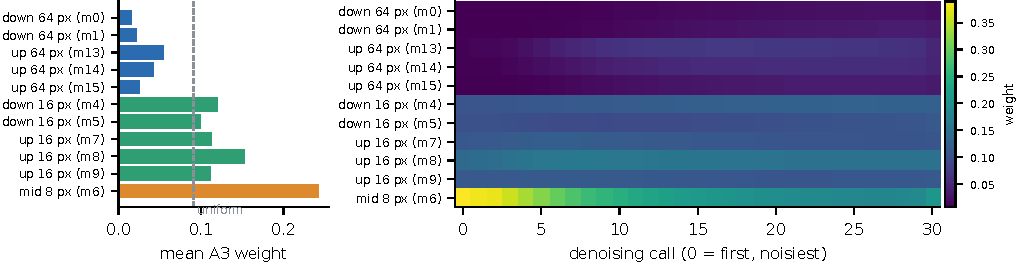
\includegraphics[width=.92\textwidth]{figures/a3_weights.pdf}
\caption{\textbf{SA-guided CA layer weights} (VOC-Sim, all images). Left: mean weight per module, against uniform weighting (dashed). Right: mean weight per denoising call. Weighting by agreement with SA moves 84\% of the weight to the 8- and 16-pixel modules.}
\label{fig:supp_a3}
\end{figure*}

\paragraph{Orientation of the agreement score.}
In our implementation, the resized SA affinity is indexed [key, query], so the score is $\langle\tilde S^\top,P\rangle$ rather than GoCA's $\langle\tilde S,P\rangle$. A paired rerun accumulated both seeds in the same diffusion run (Table~\ref{tab:supp_a3g}). The two seeds agree to Pearson 0.99999 (mean absolute difference 0.0008). The control after DenseCRF changes by $-0.0000$, inside the pre-registered $\pm0.002$ tie band, and the hierarchy's gain is unchanged on the corrected seed. All results use the historical orientation.

\begin{table}[t]
\centering
\footnotesize\setlength{\tabcolsep}{3pt}
\begin{tabular}{@{}lccc@{}}
\toprule
Cell (+ DenseCRF) & VOC forced OOF & folds vs.\ V0 & COCO \\
\midrule
historical SA-guided seed $\rightarrow$ fine only (V0) & .8228 & -- & .6623 \\
GoCA-oriented SA-guided seed $\rightarrow$ fine only (G0) & .8228 & 3/5 & .6617 \\
historical SA-guided seed $\rightarrow$ hierarchy + cap (V3) & .8292 & 5/5 & .6967 \\
GoCA-oriented SA-guided seed $\rightarrow$ hierarchy + cap (G3) & .8304 & 5/5 & .6961 \\
\bottomrule
\end{tabular}
\caption{\textbf{Orientation of the agreement score (paired rerun).} Both seeds come from the same diffusion run. G0 $-$ V0 $=-0.0000$ (CI $[-0.0001,+0.0001]$); G3 $-$ G0 $=+0.0075$ (5/5, CI $[+0.0020,+0.0128]$); G3 $-$ V3 $=+0.0012$ (4/5).}
\label{tab:supp_a3g}
\end{table}


\paragraph{The cap as a projection.}
Let $q\ge0$ be the 32-pixel proposal and $r\ge0$ the 16-pixel parent. Consider the problem
\begin{equation}
\min_{z\ge0}\ \sum_k\Big(z_k\log\frac{z_k}{q_k}-z_k+q_k\Big)\quad\text{s.t.}\quad\sum_{k\in g}z_k\le 4r_g\ \ \forall g .
\end{equation}
The objective and the constraints separate over groups. Within a group, the stationarity condition gives $z_k=q_k e^{-\lambda_g}$ with multiplier $\lambda_g\ge0$. If $\sum_{k\in g}q_k\le4r_g$, then $\lambda_g=0$ and $z=q$; otherwise the constraint is active and $e^{-\lambda_g}=4r_g/\sum_{k\in g}q_k$. This is Eq.~4 of the main paper. Replacing $\le$ by $=$ gives \emph{exact conservation}, $z_k=q_k\,4r_g/\sum_{k\in g}q_k$ for every group. That forces under-budget groups to grow as well, so children must fill a parent's budget even where the parent was wrong. A relaxed variant ($\rho{=}0.5$, Table~\ref{tab:supp_hier}) moves halfway from $q$ towards the conserved solution. The variants with conservation in Table~3 of the main paper operate on per-call distributions (each call normalized to unit mass), whereas the cap operates on the raw maps. This is why the plain hierarchy, rather than the conservation rows, is the cap's direct control: if no group binds, the capped map equals the plain hierarchy exactly.

\paragraph{DenseCRF.}
We call the SimpleCRF wrapper used by OVAM. The unary term is the hard binary mask ($p(\text{fg}){=}1$ inside, $0$ outside), and the parameters are $(w_1,\theta_\alpha,\theta_\beta,w_2,\theta_\gamma,\text{iterations})=(10,80,13,3,3,5)$ on the full-resolution RGB image. Neither these parameters nor the threshold are tuned on COCO-Cap.

\paragraph{Cost.}
All attention is captured during the 30-step generation; nothing is optimized afterwards. The seed reads eleven CA modules at every call, and the hierarchy reads three SA modules at eleven calls. Its largest operation is applying the eight $4096\times4096$ head matrices of the 64-pixel module to one map per call, which is the same operation as fine-only propagation. DenseCRF runs once per image on the CPU.
\clearpage
